\documentclass[12pt]{amsproc}
\usepackage{pgfplots}

\include{../style}

\begin{document}

\title{Blowup Algebras}

\author{Prishita Dharampal}
\date{}
\maketitle
\vspace{-0.3in}


\section{What is a Blowup?}
    
    
    \begin{wrapfigure}{r}{0.5\textwidth}
        \centering
        % If you prefer the photo, swap the tikzpicture for:
        % \includegraphics[width=.7\textwidth]{assets/EllipticCurve2D.png}
        % \begin{tikzpicture}[scale=0.85]
        %     \definecolor{curveblue}{RGB}{27,101,187}
        %     \draw[->] (-1.7,0)--(2.4,0) node[right]{\scriptsize$x$};
        %     \draw[->] (0,-2.4)--(0,2.4) node[above]{\scriptsize$y$};
        %     \draw[red!60,dashed] (-1.3,-1.3)--(1.3,1.3) node[above right]{\scriptsize$y=x$};
        %     \draw[red!60,dashed] (-1.3,1.3)--(1.3,-1.3) node[below right]{\scriptsize$y=-x$};
        %     \draw[curveblue,thick,domain=-1.55:1.55,samples=160,smooth,variable=\t]
        %         plot ({\t*\t-1},{\t*\t*\t-\t});
        %     \fill (0,0) circle (1.4pt);
        % \end{tikzpicture}

        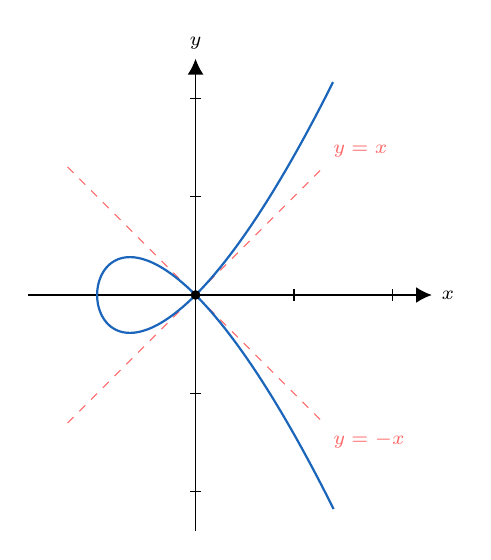
\begin{tikzpicture}[scale=1.25]
        \usetikzlibrary{arrows.meta}
        \definecolor{curveblue}{RGB}{27,101,187}

        % axes
        \draw[-{Latex[length=2mm,width=2mm]}]
            (-1.7,0)--(2.4,0) node[right]{\scriptsize $x$};

        \draw[-{Latex[length=2mm,width=2mm]}]
            (0,-2.4)--(0,2.4) node[above]{\scriptsize $y$};

        % ticks
        \foreach \x in {-1,1,2}
            \draw (\x,0.06)--(\x,-0.06);

        \foreach \y in {-2,-1,1,2}
            \draw (0.06,\y)--(-0.06,\y);

        % asymptotes
        \draw[red!60,dashed] (-1.3,-1.3)--(1.3,1.3)
            node[above right]{\scriptsize $y=x$};

        \draw[red!60,dashed] (-1.3,1.3)--(1.3,-1.3)
            node[below right]{\scriptsize $y=-x$};
        % curve
        \draw[curveblue,thick,domain=-1.55:1.55,samples=160,smooth,variable=\t]
            plot ({\t*\t-1},{\t*\t*\t-\t});

        \fill (0,0) circle (1.4pt);
    \end{tikzpicture}
        \caption{\footnotesize The nodal cubic $y^2 = x^3 + x^2$. The two branches
        cross at the origin with distinct tangent lines $y=x$ and $y=-x$.}
    \end{wrapfigure}

    We care about studying varieties, and singularities are an obstruction to that. Intuitively, a singularity is a point of the variety where the tangent is not well defined. For instance, in $\A^2$ the curve $y^2 = x^3 + x^2$ has a node at the origin, where two branches cross and there are two perfectly valid tangent directions, $y = x$ and $y = -x$.



    % \begin{tikzpicture}
    % \begin{axis}[
    %     axis lines=middle,
    %     xlabel={$x$},
    %     ylabel={$y$},
    %     samples=150,
    %     domain=-1:3,
    %     xmin=-2.2, xmax=3.2,
    %     ymin=-3.5, ymax=3.5,
    % ]
    %     \addplot[red, thick] {x*sqrt(x+1)};
    %     \addplot[red, thick] {-x*sqrt(x+1)};
    % \end{axis}
    % \end{tikzpicture}

    Blowups are a systematic tool for resolving singularities like this one. The idea is fairly straightforward, instead of picking one tangent direction at the singular point, we replace the point with a copy of $\P^1$, which parametrizes all lines through it simultaneously. The two branches then lift to the blowup as separate smooth curves, intersecting $\P^1$ at different points. 
    

    % \begin{tikzpicture}
    %     \begin{axis}[
    %         view={60}{25},
    %         xlabel={$x$},
    %         ylabel={$u$},
    %         zlabel={$y$},
    %         domain=-2:2,
    %         y domain=-2:2,
    %         samples=25,
    %         samples y=25,
    %     ]

    %     % Blowup surface y = xu
    %     \addplot3[
    %         surf,
    %         opacity=0.5,
    %     ]
    %     ({x},{y},{x*y});

    %     % Strict transform of y^2=x^2(x+1)
    %     \addplot3[
    %         very thick,
    %         red,
    %         samples=200,
    %         domain=-2:2,
    %     ]
    %     ({x^2-1},{x},{x*(x^2-1)});

    %     \end{axis}
    % \end{tikzpicture}
  
    In general, the blowup of a variety $X \subset \A^n$ at a point replaces that point with a copy of $\P^{n-1}$, thus recording all the directions one can approach it from. So it lives in $\A^n \times \P^{n-1}$. 

    Projective space $\P^n$ parametrizes lines through the origin in $\A^{n+1}$, that is, a point \\ $[p_0: p_1: \cdots : p_{n}]$ represents the line through $0$ and $(p_0, \ldots, p_n)$, with two points identified if they differ by a nonzero scalar. Thus, a polynomial $f$ only vanishes consistently at a projective point if $f(\lambda x) = 0$ whenever $f(x) = 0$, forcing $f$ to be homogeneous. Subvarieties of $\P^n$ are thus cut out by homogeneous ideals. For the homogeneous coordinate ring $k[x_0, \ldots, x_n]$ of $\P^n$, the projective Nullstellensatz correspondence sends a homogeneous radical ideal (other than the irrelevant ideal $(x_0, \ldots, x_n)$, which gives $\varnothing$) to a projective subvariety; for example,
   \begin{itemize}[topsep=2pt,itemsep=1pt]
        \item $(0)$ --- all of $\P^n$ (as a set, $\V(0) = \P^n$);
        \item $(x_i)$ --- a hyperplane $\{x_i = 0\} \iso \P^{n-1}$;
        \item $(x_i, x_j)$ --- a codimension-$2$ linear subspace $\{x_i = x_j = 0\} \iso \P^{n-2}$;
        \item $(f)$ for irreducible homogeneous $f$ of degree $d$ --- a hypersurface of dimension $n-1$.
    \end{itemize}
 

%\newpage

\section{Graded Rings and Modules}
    Since subvarieties of $\P^{n-1}$ are cut out by homogeneous ideals we need a framework to work with them. The polynomial ring $R = k[x_1, \ldots, x_n]$ decomposes naturally by degree, 
    \[R = \bigoplus_{d \geq 0} k[x_1, \ldots, x_n]_d\]
    where $R_d = k[x_1, \ldots, x_n]_d$ denotes homogeneous polynomials of degree $d$.  Multiplication respects this decomposition, $R_d \cdot R_e \subseteq R_{d+e}$, and such an $R = \bigoplus_{d \geq 0} R_d$ is called a graded ring. The polynomial ring has a natural grading by degree, but a general ring does not. To extract a graded ring from $R$, we choose ideals $I_i \subseteq R$ forming a descending multiplicative chain,
    \[R \supset I_1 \supset I_2 \supset I_3 \supset \cdots\]
    where $I_iI_j \subset I_{i+j}$. When the $I_i$ are powers of a single ideal, this chain is called an $I$-adic filtration, and it allows us to measure ``how deeply" an element lies in $I$. For our purposes, $I$ is always the maximal ideal of a local Noetherian ring $R$.

    From this filtration we can recover the associated graded ring $\gr_I R$, 
    \[\gr_I R := R/I \oplus I/I^2 \oplus I^2/I^3 \oplus \cdots,\]
    with a well-defined multiplication. For $a \in I^n/I^{n+1}$ and $b \in I^m/I^{m+1}$, we pick representatives $a' \in I^n$ and $b' \in I^m$ and define the product $ab \in I^{n+m}/I^{n+m+1}$ to be the image of $a'b'$. One can check that this is well-defined modulo $I^{m+n+1}$. We will now develop some theory around filtrations and graded rings that will be helpful later. 

    The idea of $I$-adic filtrations can be generalized to the case of modules. 
    \begin{definition}
        Given an $R$-module $M$, and an ideal $I \subseteq R$ we get the $I$-adic filtration of the module,
        \[M \supset IM \supset I^2M \supset \cdots\] 
        and the associated graded $\gr_I R$-module,
        \[\gr_I M := M/IM \oplus IM/I^2M \oplus I^2M/I^3M \oplus \cdots\]
        with multiplication defined as follows: for $a \in I^n/I^{n+1}$ and $b \in I^mM/I^{m+1}M$, we pick representatives $a' \in I^n$ and $b' \in I^mM$ and define the product $ab \in I^{n+m}M/I^{n+m+1}M$ to be the image of $a'b'$.
    \end{definition}

    \begin{definition}
        Let $R$ be a ring, $I \subseteq R$ an ideal, and $M$ an $R$-module. A filtration $M = M_0 \supset M_1 \supset \cdots$ is called an $I$-filtration if $IM_n \subseteq M_{n+1}$ for all $n \geq 0$, and $I$-stable if there exists $m$ such that $M_{m+i} = I^i M_m$ for all $i \geq 0$.
    \end{definition}

    \begin{remark}
        Note that intersecting the terms of the $I$-adic filtration of $M$ with some submodule $M' \subset M$ sadly generally does not give us the $I$-adic filtration of $M'$. 
    \end{remark}

    The Artin-Rees lemma characterizes exactly whenn this does hold. We state it now and will prove it when the requisite theory is in place. 
    
    \begin{lemma}[Artin-Rees]
        Let $R$ be a Noetherian ring, $I \subseteq R$ an ideal, and $M' \subset M$ be finitely generated $R$-modules. If
        \[M = M_0 \supset M_1 \supset M_2 \supset \cdots\]
        is an $I$-stable filtration then the induced filtration
        \[M' = M' \cap M_0 \supset M' \cap  M_1 \supset M' \cap  M_2 \supset \cdots\]
        is also $I$-stable, i.e., there exists $m$ such that $I(M' \cap M_n) = M' \cap M_{n+1}$ for $n \geq m$. 
    \end{lemma}


     
    \begin{notation}
        We write $M_k$ for $I^kM$, and
        \[\gr_I R = \bigoplus_{k \geq 0} I^k/I^{k+1}, \qquad \gr_I M = \bigoplus_{k \geq 0} M_k/M_{k+1}\]
        for the associated graded ring and module.  We also need the \emph{Rees algebra} (studied in detail in Section~\ref{blowup}) and \emph{Rees module}: for an $I$-filtration $\mathcal{J}: M = M_0 \supseteq M_1 \supseteq \cdots$,
        \[B_I R := \bigoplus_{n \geq 0} I^n t^n \subseteq R[t], \qquad B_{\mathcal{J}} M := \bigoplus_{n \geq 0} M_n\, t^n,\]
        where $B_{\mathcal{J}}M$ is a graded $B_I R$-module. (When $\mathcal{J}$ is the $I$-adic filtration, $M_n = I^n M$.)
    \end{notation}

    % \begin{proposition}
    %     Let $R$ be a ring, $I \subseteq R$ an ideal, and $M$ a finitely-generated $R$-module. If $\gr_I M = \oplus_{k \geq 0} I^k M/ I^{k+1}M$ is an $I$-stable filtration and each $I^kM/I^{k+1}M$ is a finitely-generated submodule of $M$, then $\gr_I M$ is a finitely-generated module over $\gr_I R$. 
    % \end{proposition}
    % \todo{If we need this, prove it (pg 147)}


    There is no canonical ring homomorphism $R \to \gr_I R$ lifting the structure of $R$. The only canonical ring map out of $R$ compatible with the grading is the projection onto degree $0$,
    \[R \twoheadrightarrow R/I = (\gr_I R)_0 \hookrightarrow \gr_I R,\]
    which forgets everything in positive degree. The genuinely useful gadget attached to the associated graded is instead a \emph{set} map (not a ring homomorphism), the initial form.

    % All ring maps $R \to \gr_I R$ factor over the quotient $R/I$, since any  such map must send $I$ to positive degree elements and hence $I \subset  \ker(\phi_0)$, where $\phi_0$ denotes the degree $0$ component,
    % \[\begin{tikzcd}
    %     R \arrow[r, "\phi"] \arrow[d, twoheadrightarrow] & \gr_I R \\
    %     R/I \arrow[ur, dashed, "\exists!"'] &
    % \end{tikzcd}\]
    % However there is no interesting natural homomorphism from $M$ to $\gr_I M$, but there is an interesting natural set map called the initial form.

    \begin{definition}
        Let $f \in M$ and $m$ be the greatest number such that $f \in M_m$. The intial form of $f$ is 
        \[\init(f) = f \pmod{M_{m+1}}  \in M_m/M_{m+1} \subset \gr_I M\] 
        or if $f \in \cap^\infty M_m$ 
        \[\init(f) = 0.\]
    \end{definition}
    
    \begin{definition}
        For a submodule $M' \subset M$ we define $\init(M')$ to be the $\gr_I R$-submodule of $\gr_I M$ generated by $\init(f)$ for all $f \in M'$. 
    \end{definition}

    \begin{remark}
        THe initial-form map is not additive, and it is not multiplicative when $\gr_IR$ has zero-divisors. Hence, unfortunately, $\init(M')$ is generally not obtained as the submodule generated by the initial forms of the generators of $M'$. 
        
        For instance, take $R = k[x,y]$, $I = (x,y)$, and $J = (x^2 + y^3, xy) \subset R$ with the $I$-adic filtration. The initial forms of the generators are $\init(x^2 + y^3) = x^2$ and $\init(xy) = xy$, so the submodule generated by their initial forms is $(x^2, xy) \subset \gr_I R \cong k[x,y]$. 
        However,
        \[y \cdot (x^2 + y^3) - x \cdot (xy) = x^2y + y^4 - x^2y = y^4 \in J\]
        so $\init(y^4) = y^4 \in \init(J)$. But $y^4 \notin (x^2, xy)$ in $k[x,y]$, since every element of $(x^2, xy)$ has $x$ as a factor while $y^4$ does not. Therefore $\init(J) \supsetneq (\init(x^2 + y^3), \init(xy))$.
    \end{remark}

    \begin{proposition}\label{stable}
        Let $R$ be a ring, $I \subset R$ be an ideal, and let $M$ be a finitely generated $R$-module with $I$-filtration $\mathcal{J} : M = 
        M_0 \supset M_1 \supset \cdots$ by finitely generated modules $M_i$. 
        The filtration $\mathcal{J}$ is $I$-stable if and only if the 
        $B_I R$-module $B_{\mathcal{J}}M$ is finitely generated.
    \end{proposition}

    \begin{proof}
        \bbni

        ($\implies$)

        Assume $\mathcal{J}$ is $I$-stable. Then we have $M_{n+i} = I^i M_n$ for some $n$ and all $i \geq 0$. That is, for all $k > n$, $M_k$ is generated from $M_n$ by multiplying powers of $I$. Since each $M_0, \ldots, M_n$ is finitely-generated, the union of their generating sets gives a finite generating set for $B_{\mathcal{J}}M$. 

        ($\impliedby$)

        Assume $B_{\mathcal{J}}M$ is finitely generated. Since $B_{\mathcal{J}}M = \bigoplus_{n \geq 0} M_n$ is a direct sum, every element has only finitely many nonzero homogeneous components. Therefore each generator $g_i$ is contained in $M_0 \oplus \cdots \oplus M_{k_i}$ for some finite $k_i$, and taking $n = \max(k_1, \ldots, k_r)$, all generators are contained in $M_0 \oplus \cdots \oplus M_n$. 
        
        Each generator $g_i$ decomposes as a finite sum of homogeneous pieces, and the $B_IR$-submodule generated by all these homogeneous pieces contains the $B_IR$-submodule generated by $\{g_i\}$, since each $g_i$ is a sum of its homogeneous pieces. Since $\{g_i\}$ generates $B_{\mathcal{J}}M$, the homogeneous pieces also generate $B_{\mathcal{J}}M$. Hence we may assume $B_{\mathcal{J}}M$ is generated by homogeneous elements in $M_0, \ldots, M_n$.

        Since all generators live in degrees $\leq n$, any element of $M_{n+i}$ is produced by multiplying a generator $m \in M_k$ with $k \leq n$ by some $a \in I^{n+i-k}$. Since $\mathcal{J}$ is an $I$-filtration, $I^{n-k} m \in M_n$, so $a \cdot m = I^i \cdot (I^{n-k} m) \in I^i M_n$. Therefore $M_{n+i} \subseteq I^i M_n$. The reverse inclusion $I^i M_n \subseteq M_{n+i}$ follows immediately from $\mathcal{J}$ being an $I$-filtration. Hence $M_{n+i} = I^i M_n$ for all $i \geq 0$, hence $\mathcal{J}$ is stable. 
    \end{proof}


    \begin{lemma}[Artin-Rees]
        Let $R$ be a Noetherian ring, $I \subseteq R$ an ideal, and $M' \subset M$ be finitely generated $R$-modules. If
        \[M = M_0 \supset M_1 \supset M_2 \supset \cdots\]
        is an $I$-stable filtration then the induced filtration
        \[M' = M' \cap M_0 \supset M' \cap  M_1 \supset M' \cap  M_2 \supset \cdots\]
        is also $I$-stable, i.e., there exists $m$ such that $I(M' \cap M_n) = M' \cap M_{n+1}$ for $n \geq m$. 
    \end{lemma}

    \begin{proof}
        Let 
        \[\mathcal{J}' : M' = M_0' \supset M_1' := M' \cap M_1 \supset M_2' 
        := M' \cap M_2 \supset \cdots\]
        be the induced filtration on $M'$. The module $B_{\mathcal{J}'}M' = 
        \bigoplus_{n \geq 0} (M' \cap M_n)$ is naturally a graded 
        $B_I R$-submodule of $B_{\mathcal{J}}M$. 
        
        % : for $a \in I^i$ and $m \in 
        % M' \cap M_n$ we have $am \in M'$ (since $M'$ is a submodule) and $am 
        % \in I^i M_n \subseteq M_{n+i}$ (since $\mathcal{J}$ is an 
        % $I$-filtration), so $am \in M' \cap M_{n+i}$

        Since $\mathcal{J}$ is $I$-stable, $B_{\mathcal{J}}M$ is finitely 
        generated as a $B_I R$-module by Proposition~\ref{stable}. Since $R$ is 
        Noetherian and $I$ is finitely generated, $B_I R = \bigoplus_{n \geq 
        0} I^n t^n$ is a finitely generated $R$-algebra and hence Noetherian 
        by the Hilbert basis theorem. Therefore the submodule 
        $B_{\mathcal{J}'}M'$ of the finitely generated $B_I R$-module 
        $B_{\mathcal{J}}M$ is itself finitely generated. Applying Proposition~\ref{stable} again, $\mathcal{J}'$ is an $I$-stable filtration of $M'$. 
    \end{proof}
    
    \begin{remark}
        One of the important applications of associated graded constructions is when $I = \fm$ is the maximal ideal of a Noetherian local ring, $\gr_{\fm} R$ is a finitely generated {graded} algebra over the field $R/\fm$, i.e.\ a quotient of a polynomial ring by a homogeneous ideal. Thus, $\gr_I$ allows us to turn arbitrary Noetherian rings into finitely-generated graded rings, which matters because such algebras are exactly the homogeneous coordinate rings of projective schemes, so passing to $\gr_{\fm} R$ lets us deploy the full toolkit of projective geometry ($\Proj$, Hilbert functions, Hilbert polynomials, dimension, multiplicity) on an object built from an otherwise unstructured local ring. 
        
        % Crucially, the passage $R \rightsquigarrow \gr_{\fm} R$ preserves the local numerical invariants we care about: $\dim R = \dim \gr_{\fm} R$, and the Hilbert--Samuel function $n \mapsto \ell(R/\fm^n)$ of $R$ is computed by the Hilbert function of $\gr_{\fm} R$. So dimension and multiplicity can be read off the much more tractable graded ring, and geometrically $\Spec \gr_{\fm} R$ is the tangent cone --- the linearization of $\Spec R$ at the point.
    \end{remark}

%\newpage

\section{Blow Up Algebras}\label{blowup}


\begin{definition}
    Let $R$ be a ring and $I \subseteq R$ an ideal. The \textbf{blowup algebra} (Rees algebra) of $I$ in $R$ is the $R$-algebra
    \[B_I R:= \bigoplus_{n \geq 0} I^n t^n = R \oplus It \oplus I^2t^2 
    \oplus \cdots \cong R[tI] \subset R[t]\]
    where $t$ is a formal variable tracking the degree of the ideal. The 
    associated graded ring is obtained by quotienting by $IB_IR$:
    \[B_I R/ I B_I R = \gr_I R = R/I \oplus I/I^2 \oplus \cdots \]
\end{definition}

    The blowup algebra is the algebraic structure behind the geometric operation 
    of blowing up a subvariety. Suppose $R$ is the coordinate $k$-algebra of an affine variety $X$, and $I \subset R$ is the ideal of a subvariety $Y \subset X$. Let $a_1, \ldots, a_r$ be $k$-algebra generators for $R$ and let $g_0, \ldots, g_s$ be generators of $I$ as an ideal of $R$. 
    \begin{proposition}\label{blowimage}
        The blowup algebra $B_I R$ is a homomorphic image of 
        $k[x_1, \ldots, x_r, y_0, \ldots, y_s]$.
    \end{proposition}

    \begin{proof}
        Define a ring homomorphism 
        \[\phi: k[x_1, \ldots, x_r, y_0, \ldots, y_s] \to B_I R, 
        \quad x_i \mapsto a_i, \quad y_j \mapsto g_j t\]
        This is surjective since any element of $B_I R$ is a finite sum of terms of the form $f \cdot g t^n$ with $f \in R$ and $g \in I^n$, and since $f$ is a polynomial in the $a_i$ and $g$ is a polynomial in the $g_j$, every such term is in the image of $\phi$. By the first isomorphism theorem:
        \[B_I R \cong k[x_1, \ldots, x_r, y_0, \ldots, y_s] / \ker(\phi)\]
        Since $B_IR$ is a graded ring and $\phi$ respects the grading by sending the $x_i$ to degree $0$ elements and the $y_j$ to degree $1$ elements, the kernel is a homogeneous ideal.
    \end{proof}

    Here $k[x_1,\ldots,x_r]$ is the coordinate ring of $\A^r$, and $k[y_0, \ldots, y_s]$ is the homogeneous coordinate ring of $\P^s$. So $k[x_1, \ldots, x_r, y_0, \ldots, y_s]$ is the coordinate ring of the product $A^r \times A^{s+1}$, and quotienting by a homogeneous ideal in the $y_j$ variables makes the vanishing scale-invariant in the $y_j$ and hence cuts out a subvariety that is projective in the $y$-directions, 
    \[Z = \V(\ker \phi) \subset \A^r \times \P^s\]
    The projection $\pi: \A^r \times \P^s \to \A^r$ restricts to a map $Z \to X$ which is an isomorphism away from the preimage of $Y$. The set $Z$ is called the \textbf{blowup of $Y$ in $X$}, and the preimage $\pi^{-1}(Y) \subset Z$ is called the \textbf{exceptional set}. 
    
    Algebraically, the exceptional set comes from killing $I$ inside the blowup algebra: $B_I R / I B_I R = \gr_I R$, so
    \[\pi^{-1}(Y) = \Proj(\gr_I R) \subseteq \P^s.\]
    Recall that $\gr_I R = \bigoplus_{n \geq 0} I^n/I^{n+1}$ is a graded ring, and its homogeneous primes not containing the irrelevant ideal $(\gr_I R)_{>0}$ correspond to points of a projective variety, exactly as for $k[y_0,\ldots,y_s]$ and $\P^s$. This variety --- the projectivized normal cone of $Y$ in $X$ --- parametrizes the limiting directions of approach to $Y$ inside $X$: when $Y$ is the origin in $X \subseteq \A^r$ it is the projectivized tangent cone, with one point for each limiting direction of a secant line to $X$ through $Y$. We make this precise in Section 4.

    We can now revisit the example from the start of the note more formally.


    % Algebraically, the exceptional set corresponds to:
    % \[B_I R / I B_I R = \gr_I R\]
    % The exceptional set is the projective variety associated to $\gr_I R$. Recall that $\gr_I R = \bigoplus_{n \geq 0} I^n/I^{n+1}$ is a graded ring, and its homogeneous prime ideals not containing all of $(\gr_I R)_{>0}$ correspond to points of a projective variety, exactly as homogeneous prime ideals of $k[x_0, \ldots, x_s]$ correspond to points of $\P^s$. This variety parametrizes all limiting directions of approach to $Y$ inside $X$ --- the degree $1$ piece $I/I^2$ is the space of directions, and taking its projectivization replaces $Y$ with the set of all lines through it, one for each limiting direction of a secant line to $X$ through $Y$.



    % The blowup algebra is very closely related with the blowup of a point. To see this, we revist the example from the start of this note. The curve $y^2 = x^3 + x^2$ has a singularity at the origin. To construct the blowup algebra, we have $A = \V(y^2 - x^3 - x^2 )$, and $R = k[x,y]/\langle y^2 - x^3 - x^2 \rangle$. Since we are blowing it up at the origin, the corresponding maximal ideal (by Nullstellensatz) is $I = \langle x, y \rangle$, the maximal ideal. 

    % The blowup algebra is 

    % \[B_I R:= R \oplus It \oplus I^2t^2 \cdots\]

    % which is a homomorphic image of

    % Note that the the generators of $R$ as a $k$-algebra are $\{x, y\}$ and the generators of $I$ as an ideal are also $\{x, y\}$. Relableing the latter variables gives us 

    % We are now ready to revisit the example we looked at at the start of this note more formally, 

    \subsection*{Blowing up the node of $y^2 = x^3 + x^2$}

    \begin{wrapfigure}{r}{0.5\textwidth}
        \centering
        \includegraphics[width=.5\textwidth]{assets/EllipticCurve3D_ManimCE_v0.20.1.png}
         \caption{\footnotesize Resolving the node: the slope $z=y/x$ lifts the nodal cubic to the smooth space curve $(z^2-1,\,z^3-z,\,z)$, whose two points over the origin $(z=\pm1)$ are identified under projection to the $xy$-plane.}
    \end{wrapfigure}
   

        
    The curve $X = \V(y^2 - x^3 - x^2)$ has a node at the origin. With $f = y^2 - x^3 - x^2$, the Jacobian $(\partial_x f, \partial_y f) = (-3x^2 - 2x,\; 2y)$ vanishes at $(0,0)$, and $f(0,0)=0$, so the origin is singular.

   


    % The tangent cone at the origin is computed from the lowest degree  part of $y^2 - x^3 + x^2$, which is $y^2 - x^2 = (y-x)(y+x)$, giving two  tangent lines $y = x$ and $y = -x$ as expected for a node.  
    We blow up $Y = \{0\}$ inside $X$. The coordinate ring is $R = k[x,y]/\langle y^2 - x^3 - x^2 \rangle$, and the maximal ideal of the origin is $I = \langle x, y \rangle$ (by Nullstellensatz). 
    
    Both $R$ (as a $k$-algebra) and $I$ (as an ideal) are generated by $x, y$. Relabeling the generators of $R$ as $x_1, x_2$ and the generators of $I$ as $y_0, y_1$, the blowup algebra is a homomorphic image of $k[x_1, x_2, y_0, y_1]$ by the surjection, 
    $ \phi: \begin{cases}
        x_1 \mapsto x,\\ x_2 \mapsto y, \\ y_0 \mapsto xt,\\ y_1 \mapsto yt
    \end{cases}$ by Proposition~\ref{blowimage}. 

    Two relations are visibly in $\ker\phi$: $F = x_2^2 - x_1^3 - x_1^2$, and the $G = x_1 y_1 - x_2 y_0$, since $\phi(G) = x\cdot yt - y\cdot xt = 0$. Both are homogeneous of degree $\leq 1$ in $y_0, y_1$, so they cut out a subset $Z \subseteq \A^2 \times \P^1$.
    
    To understand $Z$ as a subset of $\A^2 \times \P^1$, we cover $\P^1$ by 
    two pieces and examine $Z$ over each. Recall a point of $\P^1$ is a class 
    $[y_0 : y_1]$ under scalar identification. Every such point has either 
    $y_0 \neq 0$ or $y_1 \neq 0$, so $\P^1$ is covered by the two subsets
    \[U_0 = \{[y_0 : y_1] : y_0 \neq 0\}, \qquad 
    U_1 = \{[y_0 : y_1] : y_1 \neq 0\}.\]
    On $U_0$ we may scale the representative so that $y_0 = 1$, leaving a single 
    free coordinate $z := y_1/y_0$; this identifies $U_0$ with the affine line 
    $\A^1$ with coordinate $z$. Likewise $U_1 \cong \A^1$ with coordinate 
    $w := y_0/y_1$. We call $U_0, U_1$ the two \textbf{charts} of $\P^1$. 
    Accordingly $\A^2 \times \P^1$ is covered by $\A^2 \times U_0$ and 
    $\A^2 \times U_1$, with coordinates $(x_1, x_2, z)$ and $(x_1, x_2, w)$ 
    respectively, and we study $Z$ in each chart separately.

    \medskip
    \noindent\textbf{The chart $U_0$ (where $y_0 \neq 0$, coordinate $z = y_1/y_0$).}
    Here we may set $y_0 = 1$ and $y_1 = z$. The relation $G = x_1 y_1 - x_2 y_0$ 
    becomes
    \[x_1 z - x_2 = 0, \qquad \text{i.e.} \quad x_2 = z\, x_1.\]
    Geometrically this says exactly that $z = x_2/x_1$ is the slope $y/x$ wherever 
    $x_1 \neq 0$. Substituting $x_2 = z x_1$ into $F = x_2^2 - x_1^3 - x_1^2$ gives
    \[(z x_1)^2 - x_1^3 - x_1^2 = x_1^2\big(z^2 - x_1 - 1\big) = 0.\]
    Thus, inside the chart $\A^2 \times U_0$, the set $Z$ is cut out by
    \[x_2 = z x_1 \qquad \text{and} \qquad x_1^2\,(z^2 - x_1 - 1) = 0.\]
    The equation $x_1^2(z^2 - x_1 - 1) = 0$ factors into two pieces:
    \begin{itemize}
        \item $x_1 = 0$: this lies entirely over the origin of $\A^2$ 
        (since $x_1 = 0$ forces $x_2 = z x_1 = 0$), and is part of the 
        exceptional set $\pi^{-1}(Y)$;
        \item $z^2 - x_1 - 1 = 0$: the \textbf{strict transform}, the closure of 
        the part of $Z$ lying over $X \setminus \{0\}$.
    \end{itemize}
    On the strict transform we may solve $x_1 = z^2 - 1$, and then 
    $x_2 = z x_1 = z^3 - z$. Hence in this chart the strict transform is the 
    image of the map
    \[z \;\longmapsto\; (x_1, x_2, z) = (z^2 - 1,\; z^3 - z,\; z),\]
    which is exactly the smooth space curve of Figure~2. It is smooth because it 
    is the graph of a polynomial map in the single variable $z$.

    The points of the strict transform lying over the origin $x_1 = x_2 = 0$ 
    satisfy $z^2 - 1 = 0$, i.e. $z = \pm 1$. These are \emph{two distinct points} 
    of $Z$, with slopes $z = y/x = \pm 1$, corresponding to the two tangent 
    directions $y = x$ and $y = -x$ of the original node. The blowup has pulled 
    the two branches apart: they meet the chart's copy of $\P^1$ at the two 
    different points $z = 1$ and $z = -1$.

    \medskip
    \noindent\textbf{The chart $U_1$ (where $y_1 \neq 0$, coordinate $w = y_0/y_1$).}
    Here we set $y_1 = 1$ and $y_0 = w$. The relation $G = x_1 y_1 - x_2 y_0$ 
    becomes
    \[x_1 - x_2 w = 0, \qquad \text{i.e.} \quad x_1 = w\, x_2.\]
    Substituting into $F = x_2^2 - x_1^3 - x_1^2$ gives
    \[x_2^2 - (w x_2)^3 - (w x_2)^2 = x_2^2\big(1 - w^3 x_2 - w^2\big) = 0.\]
    Again this factors: $x_2 = 0$ lies over the origin (the exceptional set), 
    while the strict transform is $1 - w^2 - w^3 x_2 = 0$. The origin 
    $x_1 = x_2 = 0$ on the strict transform forces $1 - w^2 = 0$, i.e. 
    $w = \pm 1$, the same two tangent directions as before (note 
    $w = x/y = 1/z$, consistent with $z = \pm 1$).

    \medskip
    The two charts together cover all of $Z$, and on each the strict transform is 
    smooth. Thus the blowup $Z$ is smooth everywhere, and the single singular 
    point of $X$ has been replaced by the two points $z = \pm 1$ recording the 
    two tangent lines of the node.

   

    % To compute $Z$ explicitly, we cover $\P^1$ by two affine pieces: $U_0 = 
    % \{y_0 \neq 0\}$ and $U_1 = \{y_1 \neq 0\}$, on each of which we normalize 
    % one coordinate to $1$ and work affinely.

    % \textbf{On $U_0$} ($y_0 = 1$): We set $t = y_1/y_0$ as the affine 
    % coordinate. The relation $x_1 y_1 - x_2 y_0 = 0$ gives $y = xt$, and 
    % substituting into the curve equation:
    % \[(xt)^2 - x^3 + x^2 = 0 \implies x^2(t^2 - x + 1) = 0\]
    % The factor $x^2 = 0$ is the exceptional set sitting above the origin. Away 
    % from it, $Z \cap (\A^2 \times U_0)$ is cut out by $t^2 - x + 1 = 0$, 
    % which is smooth.

    % \textbf{On $U_1$} ($y_1 = 1$): We set $s = y_0/y_1$ as the affine 
    % coordinate. The relation $x_1 y_1 - x_2 y_0 = 0$ gives $x = ys$, and 
    % substituting into the curve equation:
    % \[y^2 - (ys)^3 + (ys)^2 = 0 \implies y^2(1 - ys^3 + s^2) = 0\]
    % The factor $y^2 = 0$ is again the exceptional set. Away from it, $Z \cap 
    % (\A^2 \times U_1)$ is cut out by $1 - ys^3 + s^2 = 0$, which is smooth.

    % The exceptional set sits above the origin and corresponds to $\gr_I R$. 
    % The degree $1$ piece $I/I^2$ is spanned by $x$ and $y$ modulo $I^2$, so 
    % the exceptional set is $\Proj(\gr_I R) \cong \P^1$. The two branches of 
    % the node meet $\P^1$ at the points $[1:1]$ and $[1:-1]$, corresponding to 
    % the tangent directions $y = x$ and $y = -x$. The blowup has separated the 
    % two branches, resolving the singularity.

    %\newpage 

    \section{Tangent Cone}

    \begin{theorem}[Krull's Intersection Theorem]
        Let $R$ be a Noetherian ring, $I \subseteq R$ an ideal, and $M$ a finitely-generated $R$-module. There exists an element $r \in I$ such that \[(1-r) \bigcap_{k=1}^\infty I^kM = 0\]
    \end{theorem}

    \begin{proof}

        Let $N = \bigcap_{k=1}^\infty I^k M$. We want to find $r \in I$ such 
        that $(1-r)N = 0$. Consider the $I$-adic filtration on $M$, 
        \[M \supset IM \supset I^2M \supset \cdots\]
        and the induced filtration on $N$, 
        \[N \supset N \cap IM \supset N \cap I^2M \supset \cdots\]
        By Artin-Rees applied to $N \subset M$, there exists $m$ such that for 
        all $n \geq m$, 
        \[N \cap I^n M = I^{n-m}(N \cap I^m M)\]
        In particular, 
        \[N \cap I^{m+1}M = I(N \cap I^m M)\]
        But since $N$ is the intersection of all $I^kM$ we have $N \subseteq I^{m+1}M$, so $N \cap 
        I^{m+1}M = N$. Similarly $N \subseteq I^m M$, so $N \cap I^m M = N$. 
        Therefore:
        \[N = IN\]
        Since $R$ is Noetherian and $M$ is finitely generated, $N$ is a 
        finitely generated $R$-module. Applying Nakayama's lemma to $N = IN$: 
        there exists $r \in I$ such that $(1-r)N = 0$.
    \end{proof}

    \begin{corollary}
        If $R$ is a Noetherian domain or $(R, \fm)$ is a local Noetherian ring, and $I \subsetneq R$ then 
        \[\bigcap_{k=1}^\infty I^k = 0\]
    \end{corollary}

    \begin{proof}
        Let $M = R$. Since $I$ is a proper ideal, there exists some $r \in I$ such that $r \neq 1$, so $1 - r \neq 0$. If $R$ is a domain, we are done. If $R$ is a local ring, $r \in I \subseteq \fm$ so $1 - r \notin \fm$, hence $1-r$ is a unit and must be non-zero. Hence, $\cap_{k=1}^\infty I^k = 0$.
    \end{proof}

    \begin{corollary}
        If $R$ is a Noetherian local ring and $I \subsetneq R$ is an ideal then if $\gr_I R$ is a domain, so is $R$.  
    \end{corollary}

    \begin{proof}
        If $fg = 0 \in R$ then $\init(f) \init(g) = 0 \in \gr_I R$. Since $\gr_I R$ is a domain, $\init (f)$ or $\init(g)$ is zero. Without loss of generality, assume $\init(f) = 0$. Then by definition, $f \in \cap_{k=1}^\infty I^k$ and by KIT we know that $\cap_{k=1}^\infty I^k = 0$. Hence $f = 0$. Thus, $R$ is a domain. 
    \end{proof}

    We now make the link between the exceptional set and the associated graded ring geometric. Throughout, $R = k[x_1, \ldots, x_r]/J$ with $I = (x_1, \ldots, x_r)$, $k$ algebraically closed, and $J \subseteq I$ (so the origin lies on $X$); let $X = \V(J) \subseteq \A^r$. 

    The correspondence between the exceptional set in the blow up and the associated graded ring gives us a beautiful geometric consequence. 
     \begin{definition}
        A line through $0$ in $\mathbb{A}^r$ is determined by its direction, a point of
        $\mathbb{P}^{r-1}$: the line through $0$ and $p=(p_1,\dots,p_r)$ corresponds to
        $[p_1:\cdots:p_r]\in\mathbb{P}^{r-1}$. A secant line to $X$ through $0$ has the
        form $\overline{0p}$ with $p\in X\setminus\{0\}$, giving a direction
        $[p]\in\mathbb{P}^{r-1}$, and a \emph{limiting secant direction} is a limit point
        \[
        [p]=\lim_{n\to\infty}[p_n],\qquad p_n\in X\setminus\{0\},
        \]
        which exists after passing to a subsequence since $\mathbb{P}^{r-1}$ is compact. Let
        \[
        D \;=\; \overline{\{\,[p]\in\mathbb{P}^{r-1} : p\in X\setminus\{0\}\,\}}
            \;\subseteq\;\mathbb{P}^{r-1}
        \]
        denote the closure of the set of these directions. The \emph{(affine) tangent cone}
        of $X$ at $0$ is the cone over $D$,
        \[
        TC_0(X)\;=\;\{0\}\;\cup\;\{\,x\in\mathbb{A}^r\setminus\{0\} : [x]\in D\,\}
                \;\subseteq\;\mathbb{A}^r,
        \]
        the union of all lines through the origin in the limiting directions. Taking the
        closure is essential because it adds directions that arise as limits of secants but are not themselves the direction of any point of $X\setminus\{0\}$.
    \end{definition}

    % \begin{definition}
    %     A line through $0$ in $\A^r$ is determined by its direction (which corresponds to a point in $\P^{r-1}$). More precisely, the line through $0$ and $p = (p_1, \ldots, p_r)$ corresponds to $[p_1 : \cdots : p_r] \in \P^{r-1}$
    %     So a sequence of secant lines $\ell_{p_n}$ at a variety $X \subset A^r$ is really a sequence of points $[p_n] \in \mathbf{P}^{r-1}$. A \textbf{limiting position} is a limit point of this sequence:
    %     $$\ell = \lim_{n \to \infty} [p_n] \in \P^{r-1}$$
    %     This is well-defined because $\P^{r-1}$ is compact, so every sequence has a convergent subsequence.
    % \end{definition}

    We define the tangent cone of $X$ at $0$ as the cone composed of all lines that are the limiting positions of secant lines to $X$ passing through the point $0$. Alternatively, the tangent cone at $0$ is then the closure of the set of directions of points on $X$, together with the actual lines they represent in $\A^r$. 
    \[TC_0(X) = \overline{\{[p] \in \mathbf{P}^{r-1} : p \in X \setminus \{0\}\}} \subset \mathbf{P}^{r-1}\]
    The closure captures limiting directions that arise as limits of secant lines but may not themselves be the direction of a point of $X \setminus \{0\}$.
    
    \begin{definition}
        The set of limiting secant directions,
        \[
        PTC_0(X)\;:=\;\overline{\{\,[p] : p\in X\setminus\{0\}\,\}}\;\subseteq\;\mathbb{P}^{r-1},
        \]
        is the \emph{projectivized tangent cone}; it is the set $D$ of Definition 4.2.
        Over $\mathbb{C}$ the closure is genuinely a set of limits: if $p_n\in X\setminus\{0\}$
        with $p_n\to 0$, the directions $[p_n]$ have a convergent subsequence because
        $\mathbb{P}^{r-1}$ is compact. The affine tangent cone $TC_0(X)\subseteq\mathbb{A}^r$
        is the cone over $PTC_0(X)$, and $PTC_0(X)$ is precisely the exceptional set of
        $\mathrm{Bl}_0 X$ from Section 3.
    \end{definition}

    % \begin{definition}
    %     A point $p = (p_1,\ldots,p_r) \in \A^r \setminus \{0\}$ spans a secant line $\overline{0p}$, i.e.\ a direction $[p_1 : \cdots : p_r] \in \P^{r-1}$. The set of \emph{limiting} secant directions,
    %     \[\P TC_0(X) := \overline{\{[p] : p \in X \setminus \{0\}\}} \subseteq \P^{r-1},\]
    %     is the \textbf{projectivized tangent cone}. Over $\C$ the closure is genuinely a set of limits: if $p_n \in X\setminus\{0\}$ with $p_n \to 0$, the directions $[p_n]$ have a convergent subsequence because $\P^{r-1}$ is compact. The \textbf{(affine) tangent cone} $TC_0(X) \subseteq \A^r$ is the cone over $\P TC_0(X)$ --- the union of all these lines through the origin (together with $0$). It is the affine version, and the object the theorem below describes; its projectivization $\P TC_0(X)$ is precisely the exceptional set of $\Bl_0 X$ from \S3.
    % \end{definition}


    % One can show that the ideal $\ini_I(J) \subset k[x_1, \ldots, x_r]$ defines the tangent cone so that the coordinate ring of the tangent cone is $\gr_{(x_1, \ldots, x_r)}R$. \todo{exercise 5.3 eisenbud}


% \section{Conclusion} 

%     \todo{Talk about}
% %\newpage 

% \section{Worksheet} 

%  \todo{Add figure and theorem}

    \begin{theorem}
    Let $R = k[x_1, \ldots, x_r]/J$ with $I = (x_1, \ldots, x_r)$ and 
    $k$ algebraically closed. The tangent cone $TC_0(X)$ to $X = \V(J) 
    \subset \A^r$ at the origin is the algebraic subset:
    \[TC_0(X) = \V(\init_I(J)) \subset \A^r\]
    where $\init_I(J) = \langle \init(f) : f \in J \rangle \subset k[x_1, \ldots, x_r]$ 
    is the ideal generated by the initial forms of all elements of $J$. 
    Moreover, the coordinate ring of the tangent cone is:
    \[k[x_1, \ldots, x_r]/\init_I(J) \cong \gr_I R\]
    \end{theorem}

% \begin{proof}
%     We sketch the key steps; for a complete proof see Harris
    
%     First, $\init_I(J)$ is a homogeneous ideal since each $\init(f)$ is 
%     homogeneous by definition, so $\V(\init_I(J))$ is indeed a cone in 
%     $\A^r$.

%     For the geometric identification: a direction $[v] \in \P^{r-1}$ lies 
%     in $TC_0(X)$ if and only if $v$ is a limit of directions $[p_n]$ with 
%     $p_n \in X \setminus \{0\}$ and $p_n \to 0$. Writing $p_n = t_n v_n$ 
%     with $t_n \to 0$ and $v_n \to v$, and expanding $f(t_n v_n) = 0$ for 
%     $f \in J$, the leading order term gives $\init(f)(v) = 0$. Since this 
%     holds for all $f \in J$, we get $v \in \V(\init_I(J))$. The converse 
%     holds by a similar limiting argument.

%     For the ring isomorphism, note that the natural map:
%     \[k[x_1, \ldots, x_r] \twoheadrightarrow \gr_I R = \bigoplus_{n \geq 
%     0} I^n/I^{n+1}\]
%     sending $x_i$ to its class in $I/I^2$ is surjective with kernel 
%     $\init_I(J)$, giving $\gr_I R \cong k[x_1, \ldots, x_r]/\init_I(J)$.
% \end{proof}

\begin{proof}[Proof sketch]
    The theorem has two halves, algebraic and geometric, and the algebraic half  does most of the work.

    For the algebraic statement, write $S = k[x_1, \ldots, x_r]$ and 
    $\fm = (x_1, \ldots, x_r) \subset S$, so $R = S/J$ and $I = \fm R$. The polynomial ring is its own associated graded for the $\fm$-adic 
    filtration: the quotient $\fm^n/\fm^{n+1}$ is naturally identified with the 
    space $S_n$ of degree-$n$ forms (a polynomial in $\fm^n$ is remembered modulo 
    $\fm^{n+1}$ only through its lowest, degree-$n$ part), so $\gr_{\fm} S \cong S$.
    Since $I^n = (\fm^n + J)/J$, the induced surjection  $S \cong \gr_{\fm} S \twoheadrightarrow \gr_I R$ has kernel exactly the ideal 
    generated by the initial forms $\init(f)$, $f \in J$, namely $\init_I(J)$. 
    Hence
    \[\gr_I R \cong S/\init_I(J) = k[x_1, \ldots, x_r]/\init_I(J).\]
    % By the Remark in \S2, $\init_I(J)$ is \emph{not} generated by the initial 
    % forms of a generating set of $J$, so the kernel must be computed using all 
    % of $J$.

    For the geometric statement $TC_0(X) = \V(\init_I(J))$, one inclusion is obvious: if $f \in J$, then $\init(f)$ vanishes on every limiting secant direction, giving $TC_0(X) \subseteq \V(\init_I(J))$. The reverse inclusion uses the fact that $k$ is algebraically closed; we omit 
    it, as a rigorous argument needs limiting tools beyond these notes. The worksheet walks through the rest of this proof in detail. 
\end{proof}

\begin{wrapfigure}{r}{0.45\textwidth}
    \centering
    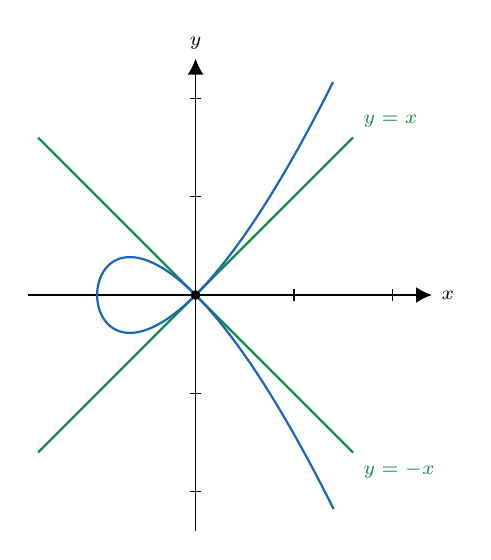
\begin{tikzpicture}[scale=1.25]
    \usetikzlibrary{arrows.meta}
    \definecolor{curveblue}{RGB}{27,101,187}
    \definecolor{conegreen}{RGB}{20,140,70}

    % axes
    \draw[-{Latex[length=2mm,width=2mm]}]
        (-1.7,0)--(2.4,0) node[right]{\scriptsize $x$};
    \draw[-{Latex[length=2mm,width=2mm]}]
        (0,-2.4)--(0,2.4) node[above]{\scriptsize $y$};

    % ticks
    \foreach \x in {-1,1,2}
        \draw (\x,0.06)--(\x,-0.06);
    \foreach \y in {-2,-1,1,2}
        \draw (0.06,\y)--(-0.06,\y);

    % tangent cone: the two lines y = x and y = -x
    \draw[conegreen,thick] (-1.6,-1.6)--(1.6,1.6)
        node[above right]{\scriptsize $y=x$};
    \draw[conegreen,thick] (-1.6,1.6)--(1.6,-1.6)
        node[below right]{\scriptsize $y=-x$};

    % nodal cubic y^2 = x^3 + x^2
    \draw[curveblue,thick,domain=-1.55:1.55,samples=160,smooth,variable=\t]
        plot ({\t*\t-1},{\t*\t*\t-\t});

    \fill (0,0) circle (1.4pt);
    \end{tikzpicture}
    \caption{\footnotesize The tangent cone $TC_0(X) = \V(y^2 - x^2)$ is the pair of lines $y = \pm x$, matching the two branches' 
    tangent directions and the two points $z = \pm 1$ found in the blowup 
    of Section 3.}
\end{wrapfigure}

Revisiting the example we have been working with, for the nodal curve $y^2 = x^3 + x^2$, the lowest degree part of  $f = y^2 - x^3 - x^2$ is $\init_I(f) = y^2 - x^2 = (y-x)(y+x)$. So the tangent cone is $\V(y^2 - x^2) \subset \A^2$, the union of the two lines $y = x$ and $y = -x$, confirming the two tangent directions at the node. The coordinate ring is $k[x,y]/(y^2 - x^2) \cong \gr_I R$.

We can now see the full picture for the node. In Section 1 we promised that  blowing up replaces the singular point by a $\P^1$ recording tangent directions; in Section 3 we made this concrete, lifting the nodal cubic to a smooth curve whose two points $z = \pm 1$ over the origin record the two 
branches; and in this section we identified those directions purely algebraically. The three descriptions agree: the tangent cone 
$\V(\init_I f) = \V(y^2 - x^2)$ is the pair of lines $y = \pm x$, its projectivization $\{[1{:}1], [1{:}{-}1]\} \subset \P^1$ is the exceptional set of the blowup, and its coordinate ring is $\gr_I R$.
\par\noindent\ignorespaces
\clearpage

\newpage 


% \section{Worksheet}

% Throughout, let $S = k[x_1, \ldots, x_r]$ with $k$ algebraically closed,  $\fm = (x_1, \ldots, x_r)$, let $J \subseteq \fm$ be an ideal, $R = S/J$, $X = \V(J) \subseteq \A^r$, and $I = \fm R$. The goal of this worksheet is to prove 
% \[\gr_I R \;\cong\; S/\init_I(J)\]
% and to verify the easy half of the geometric statement on a concrete example.

% \begin{problem}{1} \textbf{The Graded Pieces.}

%     \begin{enumalph}
%         \item Show that $I^n = (\fm^n + J)/J$ as ideals of $R = S/J$. 
%         \emph{(Hint: $I = \fm R$ is generated by the images of $x_1, \ldots, x_r$; 
%         describe $I^n$ as the image of $\fm^n$ under $S \twoheadrightarrow R$.)}

%         \item Using part (a), establish the isomorphism of $k$-vector spaces
%         \[\frac{I^n R}{I^{n+1} R} \;\cong\; \frac{\fm^n + J}{\fm^{n+1} + J}.\]
%         \emph{(Hint: apply the third isomorphism theorem to the quotient of 
%         quotients.)}

%         \item The polynomial ring $S$ is graded by degree, $S = \bigoplus_n S_n$ 
%         where $S_n$ is the span of degree-$n$ monomials. Show that 
%         $S_n \cong \fm^n/\fm^{n+1}$ as $k$-vector spaces, and conclude that 
%         $\gr_{\fm} S \cong S$ as graded rings. 
%     \end{enumalph}
% \end{problem}

% \begin{problem}{2} \textbf{Initial Forms}
%     \begin{enumalph}     
%         \item Recall from Section 2 that for $f \in S$ with $f \in \fm^m \setminus  \fm^{m+1}$, the initial form $\init(f) \in \fm^m/\fm^{m+1} = S_m$ is the  lowest-degree homogeneous part of $f$. Define a graded ring  homomorphism 
%         \[\phi : S \cong \gr_{\fm} S \longrightarrow \gr_I R, \qquad  S_n \ni \overline{g} \longmapsto \big(g + \fm^{n+1} + J\big)  \in \frac{I^n R}{I^{n+1}R}.\] 
        
%         Using Problem 1, show that $\phi$ is surjective.  

%         \item Show that for $g \in S_n$ (homogeneous of degree $n$), 
%         \[g \in \ker \phi \iff g \in \fm^{n+1} + J\] 
%         Then show that $(\ker(\phi))_n = \init_I(J) \cap S_n$ and thus deduce that $\ker\phi = \init_I(J)$, the ideal generated by 
%         $\{\init(f) : f \in J\}$.

%         \item Conclude from parts (a) and (b) that
%         \[\gr_I R \cong S/\init_I(J).\]

%         \item \emph{(Why all of $J$ is needed.)} Revisit the Remark in Section 2 with 
%         $J = (x^2 + y^3, xy) \subset k[x,y]$. Show that $y^4 \in \init_I(J)$ but 
%         $y^4 \notin (\init(x^2+y^3), \init(xy)) = (x^2, xy)$. Explain why this 
%         means $\gr_I R$ \emph{cannot} be computed by only taking initial forms 
%         of a chosen generating set of $J$. 
%     \end{enumalph}
% \end{problem}

% \newpage

% \begin{problem}{3}
%     \begin{enumalph}
%         \item Let $f \in J$ with initial form $\init(f) = f_m$ (its degree-$m$ part, $f_m \neq 0$), so $f = f_m + f_{m+1} + \cdots + f_d$ with each $f_i$ homogeneous of degree $i$. Fix a nonzero direction $p = (p_1, \ldots, p_r)$ and consider the points $tp \in \A^r$ for $t \in k$. Compute $f(tp)$ as a polynomial in $t$ and show \[f(tp) = t^m\big(f_m(p) + t\, f_{m+1}(p) + \cdots + t^{d-m} f_d(p)\big).\]

%         \item Suppose $p_n \in X \setminus \{0\}$ is a sequence with $p_n \to 0$ 
%         and $[p_n] \to [p]$ in $\P^{r-1}$. Using that $f(p_n) = 0$ for all $n$ 
%         (since $p_n \in X$ and $f \in J$), argue informally that $f_m(p) = 0$, 
%         i.e.\ the limiting direction $[p]$ lies in $\V(\init(f))$. Conclude 
%         \[TC_0(X) \subseteq \V(\init_I(J)).\]
%         \emph{(This is the easy inclusion. The reverse inclusion holds when $k$ 
%         is algebraically closed but requires tools beyond these notes.)}

%         \item \emph{(Worked example.)} For $f = y^2 - x^3$, the cuspidal cubic curve, carry out part (a) explicitly: find $\init(f)$, factor it, and identify the limiting secant direction in $\P^1$.
%     \end{enumalph}
% \end{problem}


\section*{References and Credits}
This note closely follows Eisenbud, \emph{Commutative Algebra with a View 
Toward Algebraic Geometry}, and refers to Harris, \emph{Algebraic 
Geometry: A First Course}. The illustrations are courtesy of Sair 
Shaikh~'26.

% \begin{problem}{1}

% \end{problem}

% \begin{enumerate}
%     \item Motivation 
%     % \item Graded Rings \& Modules 
%     % \item Filtrations, Stable Filtrations, Initial forms, Artin-Rees
%     \item KIT 
%     \item Blow Ups, Blow Up Algebras, Exceptional Sets 
%     \item Limiting Points and Tangent Cones
%     \item Flatness 
%     \item Projective and Free Resolutions 
%     \item `Criteria for Flatness'
%     \item Rees Algebras
% \end{enumerate}

% \begin{enumerate}
    % \item \todo{Motivation}
    % \item Homogeneus prime ideals encode homogeneus polynomials vanishing on some projective subvariety of the ring. For instance, given the (homogeneous coordinate) ring $k[x_0, \ldots, x_n]$, in its associated  projective space $P^n = \Proj(k[x_0, \ldots, x_n])$ we have
    % \begin{itemize}
    %     \item $(0)$ — corresponds to all of ${\P}^n$
    %     \item $(x_i)$ — a hyperplane $\{x_i = 0\} \iso P^{n-1}$
    %     \item $(x_i, x_j)$ — a codimension-2 linear subspace $\{x_i, x_j = 0\} \iso P^{n-2}$
    %     \item $(f)$ for homogeneous irreducible $f$  of degree $d$ - a hypersurface $\iso P^{n-d}$. 
    % \end{itemize}
    % \item We want homogeneous primes because in $\P^n$ coordinates are only defined upto scaling. So a polynomial $f$ only vanishes consistently at a projective point if $f(\lambda x) = 0$ whenever $f(x) = 0$, which forces $f$ to be homogeneous. 
    % \item Graded Rings. 
    % \begin{itemize}
    %     \item Worth noting that all ring maps from $R \to \gr_IR$ map through the quotinent $R/I$.
    %     \item The blow up algebra surjects onto $\gr_I R$, 
    %     \[B_IR/IB_I R \iso \gr_IR\]
    %     \item If $\gr_IR$ is a domain, then $R$ is a domain (converse not true). 
    % \end{itemize}
    % \item Let $M$ be a smooth manifold and $k$ be a field. $\mathcal C^\initty(M)$ is the ring of infinitely differentiable (smooth) functions $f: M \to k$.
    % \item Let $X$ be a topological space, $x \in X$ a point, and maps $f, g: X \to k$, then $f$ and $g$ are equivalent if they agree on some open neighborhood $U$ of $x$ such that 
    % \[f \sim_x g \iff f \big |_{U}(u) = g \big |_{U}(u), \, \forall u \in U\]
    % The germ of $f$ at $x$ is its equivalence class $[f]_x$.
    % \item The ring of germs at $x$ is,
    % \[\mathcal{O}_{X, x} = \{[f]_x \mid f : U \to k\}\]
    % with addition and multiplication defined representativewise. 
    % This is a local ring with maximal ideal 
    % \[\fm_x = \{[f]_x \in \cO_{X, x} \mid f(x) = 0\}\]
    % which is maximal because evaluation at $x$ gives a surjective ring homomorphism:
    % \[\text{ev}_x: \mathcal{O}_{X,x} \twoheadrightarrow k, \quad [f]_x \mapsto f(x)\]
    % with kernel $\fm_x$, so $\cO_{X, x} / \fm_x \iso k$, which is a field. 
    % \item
    % \item \todo{Graded Rings/Modules}
    % \item \todo{Filtrations, Stable Filtrations, Initial forms, Artin-Rees}
    % \item \todo{Blow-up Algebras, Blow Ups, Exceptional Set}
    % \item Limiting point of a line: 

    % A line through $0$ in $\A^r$ is determined by its direction (which corresponds to a point in $\P^{r-1}$). More precisely, the line through $0$ and $p = (p_1, \ldots, p_r)$ corresponds to:
    %     \[[p_1 : \cdots : p_r] \in \P^{r-1}\]
    % So a sequence of secant lines $\ell_{p_n}$ is really a sequence of points $[p_n] \in \mathbf{P}^{r-1}$. A \textbf{limiting position} is a limit point of this sequence:
    % $$\ell = \lim_{n \to \infty} [p_n] \in \P^{r-1}$$
    % This is well-defined because $P^{r-1}$ is compact (over $\C$), so every sequence has a convergent subsequence.

    % \item The correspondence between the exceptional set in the blow up and the associated graded ring gives us a beautiful geometric consequence. Let $R = k[x_1, \ldots, x_r]/J$ and $I = (x_1, \ldots, x_r)$ where $k$ is algebraically closed and $J \subset I$, also let $X = \V(J) \subset \A^r$ so $0 \in X$. 
    
    % -- basically $X$ is the algebraic subset of $\A^r$ cut out by $J$. 

    % Then we define the tangent cone of $X$ at $0$ as the cone composed of all lines that are the limiting positions of secant lines to $X$ passing through the point $0$. Alternatively, the tangent cone at $0$ is then:
    % \[TC_0(X) = \overline{\{[p] \in \mathbf{P}^{r-1} : p \in X \setminus \{0\}\}} \subset \mathbf{P}^{r-1}\]
    % the closure of the set of directions of points on $X$, together with the actual lines they represent in $\A^r$. The closure is what captures the limiting directions — directions you can approach but which may not themselves be realized by points of $X \setminus \{0\}$. One can show that the ideal $\ini_I(J) \subset k[x_1, \ldots, x_r]$ defines the tangent cone so that the coordinate ring of the tangent cone is $\gr_{(x_1, \ldots, x_r)}R$. \todo{exercise 5.3 eisenbud}
    
    % \begin{itemize}
    %     \item The tangent cone at a smooth point is the tangent line. 
    %     \item 
    % \end{itemize}

    % \item \todo{Examples}

    % \item What makes a good family? Flatness! 
    % \begin{itemize}
    %     \item Algebraically, this means that when the family is represented by a $R$-algebra $S$, then $S$ is flat as a $R$-module. 
    %     \item Geometrically this means that when the family is represented by a morphism $\phi: X \to B$, then for each point $x \in X$ there is an affine neighborhood $U$ of $x$ and a affine neighborhood of $\phi(x)$ such that $\phi$ restricts to a map $U \to V$ and the corresponding map of coordinate rings $K[V] \to K[U]$ makes $K[U]$ into a flat $K[V]$-module. 
    % \end{itemize}

    % \item Free resolution helps "standardize" the sequence so tor can give us a measure of the faliure of exactness \todo{examples and definitions}
    % \item \todo{Criteria for Flatness.}
    % \item \todo{Rees Algebras as a flat family. }
% \end{enumerate}

\end{document}